\chapter{Environnement de travail et choix des outils}
\label{sec:env}

%%%%%%%%%%%%%%%%%%%%
%%% Organisation %%%
%%%%%%%%%%%%%%%%%%%%
\section{Organisation}
    \paragraph{} Pour développer ce projet, nous nous sommes organisés de la manière suivante. Tous les lundi après-midi nous nous retrouvions au LIRMM à partir de 14h et jusqu'à 18h-19h. Nous faisions le point avec notre encadrant, M. \textsc{Bourreau}. Au niveau de la répartition du travail, nous avons réalisé la plupart des tâches ensemble. Un groupe de deux personnes permet de travailler assez facilement ensemble tout en offrant la possibilité de faire des recherches chacun de son côté si besoin. En plus des réunions hebdomadaires au LIRMM, nous avons fait des recherches et programmé chez nous. Nous avions chacun en notre possession quelques capteurs et cartes de développement, ce qui nous a permis de réaliser des tests chez nous.\\
    Étant dans le même groupe de Licence tous les deux, il nous était aussi possible de communiquer et d'échanger régulièrement durant toute la semaine.


%%%%%%%%%%%%%%%%%%%%
%%% API de m***e %%%
%%%%%%%%%%%%%%%%%%%%
\section{Environnement logiciel (API)}
    \paragraph{}Libelium fournit un environnement de développement (IDE) multi-plateforme et une API consultable sur son site internet. L'IDE est très similaire à celui de la société Arduino qui propose des cartes de développement à bas coût (voir figure \ref{fig:ide}). Le langage nécessaire à la programmation est le C++. Néanmoins, toutes les fonctionnalités du C++ ne sont pas disponibles : l'allocation de mémoire dynamique n'est pas autorisée ; il est par conséquent impossible de s'appuyer sur les conteneurs de la bibliothèque standard qui utilisent l'allocation dynamique de manière interne (comme les Vector). 
    
    \paragraph{}On y retrouve les éléments caractéristiques de la programmation Arduino. Pour compiler le code, il est nécessaire d'ajouter deux fonctions. Tout d'abord la fonction {\bfseries\color{black!70}\textit{setup()}} qui ne sera parcourue qu'une seule fois au lancement du programme ; il faut insérer dans cette partie tout ce qui doit être vérifié ou initialisé au démarrage du programme. Vient enfin la fonction {\bfseries\color{black!70}\textit{loop()}} qui sera parcourue en boucle jusqu'à la fin du programme. C'est dans cette boucle que la majorité du programme est conçu.
    
    \paragraph{}Sur le site internet de Libelium se trouve toute l'API des Waspmotes. Elle renseigne la définition et le code source de toutes les fonctions et classes nécessaires à la programmation et bonne exécution du code. Cependant, il est difficile de s'y retrouver et il nous a paru compliqué de s'aider de cette API pour le développement. Heureusement, le guide technique fourni par Libelium donne les fichiers et classes importants pour pouvoir programmer. De plus, l'IDE intègre de très nombreux exemples de code qui sont classés en différentes catégories. Cela facilite grandement la compréhension de la programmation sur Waspmotes et les exemples peuvent être utilisés et complétés facilement.
    
     \begin{figure}[h]
        \centering
        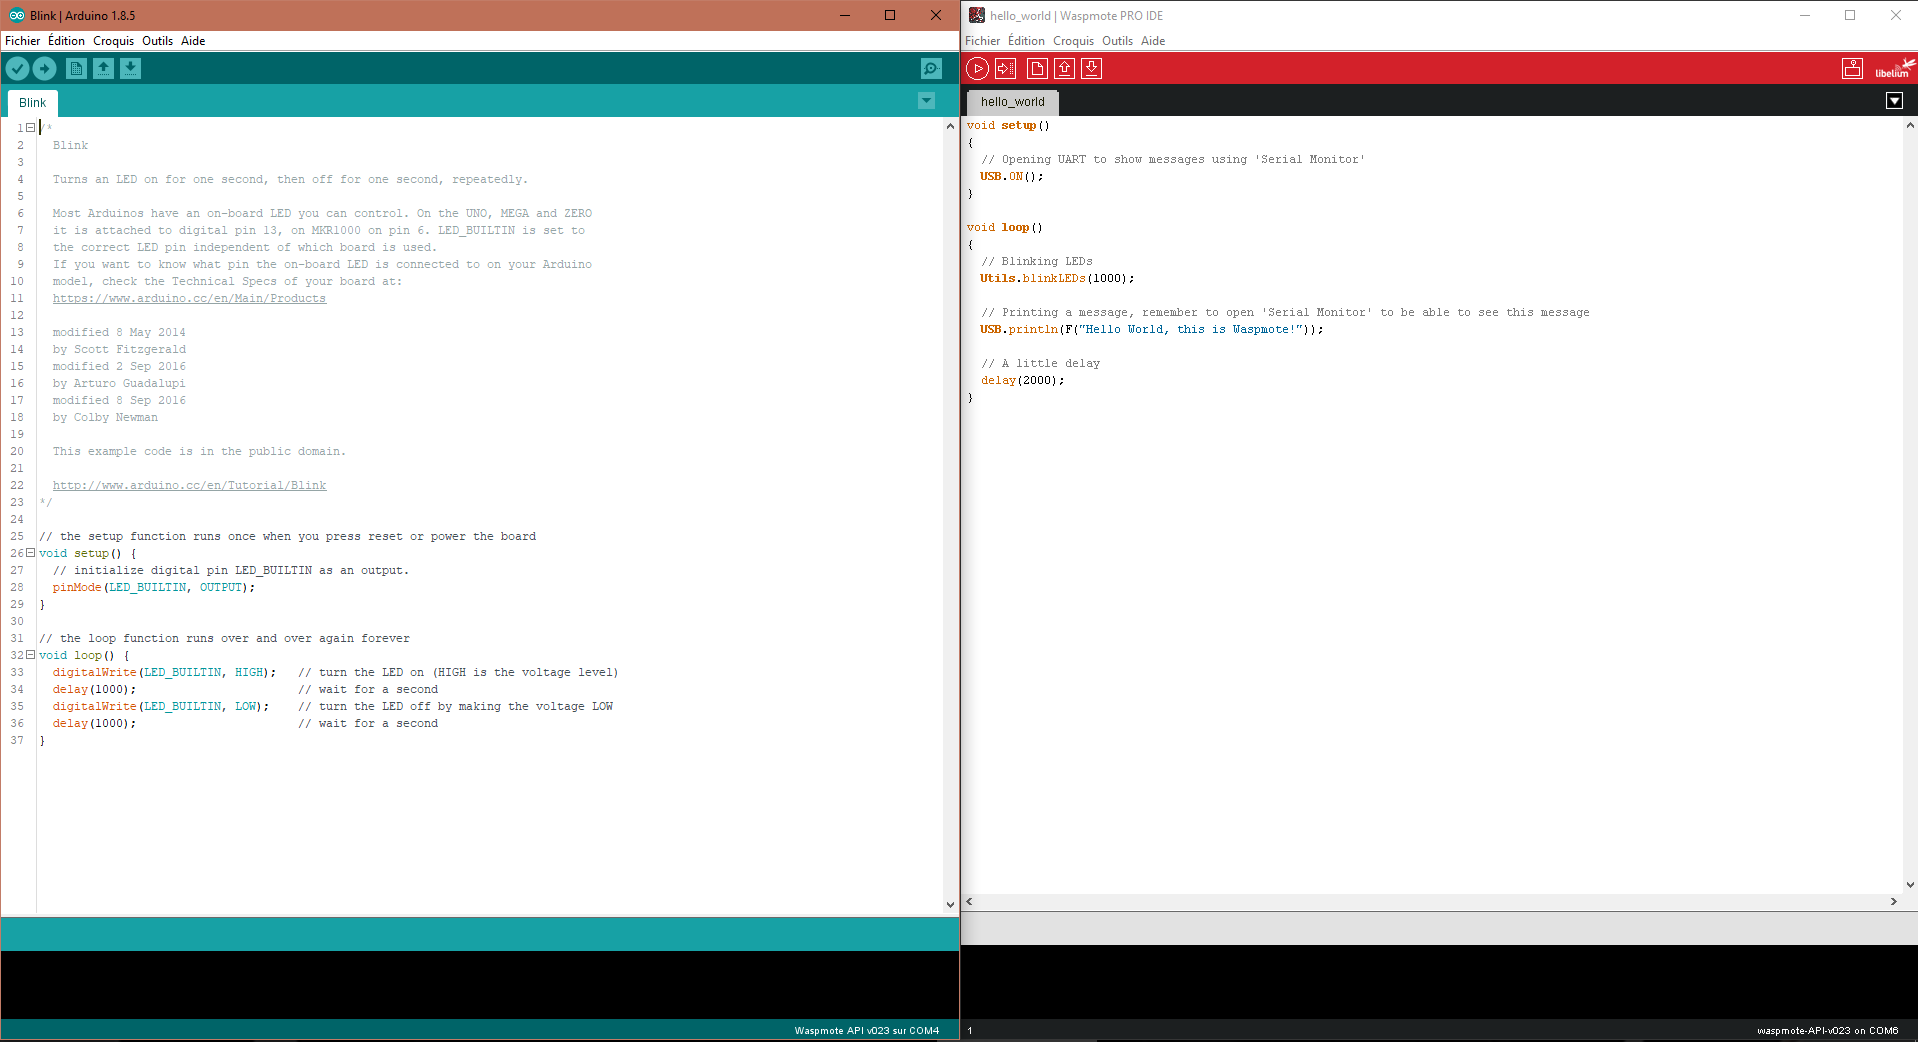
\includegraphics[scale=0.25]{images/photos/ide.png}
        \caption{Comparaison des deux IDE, l'original à gauche et Libelium à droite.}
        \label{fig:ide}
    \end{figure}
    
    \paragraph{}La communication entre les cartes de développement et l'IDE installé sur l'ordinateur se fait par liaison USB. L'IDE permet de compiler les programmes et de les téléverser sur les cartes. Il intègre aussi une sorte de console qui permet d'afficher si on le souhaite des caractères depuis les Waspmotes. Cela permet ainsi de vérifier des données ou des variables et d'avoir un retour sur le fonctionnement du programme sur la Waspmote. L'IDE permet également la coloration syntaxique du code. En revanche, il ne présente pas de fonctionnalités d'auto-complétion ou de suggestion. Il est néanmoins possible d'utiliser d'autres IDE présentant ces fonctionnalités et pouvant être compatibles avec les Waspmotes après paramétrage (testé sur Visual Code Studio par exemple).
    
    
%%%%%%%%%%%%%%%%
%%% Matériel %%% 
%%%%%%%%%%%%%%%%
\section{Matériel}
    \paragraph{}Afin de mener à bien ce projet, nous avons à notre disposition plusieurs microcontrôleurs : les Waspmotes (cf. \ref{tab:modules}) ainsi que toute une panoplie de capteurs (cf. \ref{tab:capteurs}). Les Waspmotes bien qu'étant d'ancienne génération --- Libelium ayant depuis sorti 2 nouvelles versions~--- permettent une prise en main de l'écosystème Libelium. Ainsi nous avons pu effectuer différents tests, notamment sur quelques capteurs ainsi que sur la transmission d'informations basiques entre les capteurs. Nous n'avons pas été en mesure de tester l'intégrité des données lors des transferts en raison de plusieurs difficultés qui ont engendré un manque de temps.
    
    \paragraph{}Le matériel à notre disposition peut être décomposé en deux principales catégories que sont \emph{capteurs} et les \emph{les microcontrôleurs}. Les premiers se connectent aux seconds via des pins dédiés ainsi qu'à l'aide de cartes connecteurs nécessaires à certain capteur.\\
    L'avantage majeur de cette décomposition en carte mère / capteurs est la modularité que cela permet. En effet, cette séparation des priorités permet l'ajout simple d'un capteur sans modification majeure du code initial. De plus, à condition d'avoir initialement anticipé un minimum l'évolutivité du réseau, l'ajout d'un n\oe ud à celui-ci se fait de façon tout aussi naturelle.
    
    \subsection{Modules de communication}
        \paragraph{}Différents modules de communications fournis par Libelium ont été présentés au sein la \textit{partie \ref{chap:etat-art}}. Comme indiqué précédemment, nous avions déjà du matériel à notre disposition dont la liste des capteurs se trouve tableau \ref{tab:modules}. Les modules de communication compris dans ce matériel sont des XBee-PRO EU et utilisent le protocole Zigbee. Nous avons donc prévu de réaliser ce projet à l'aide la technologie Zigbee par soucis de compatibilité (et afin d'éviter de racheter du matériel). 
        Nous n'oublions pas néanmoins le protocole LoRaWAN qui semble intéressant. Nous n'avons malheureusement pas ce type de module en notre possession et il est donc impossible de réaliser des tests.
        
    
    \begin{figure}[h]
        \centering
        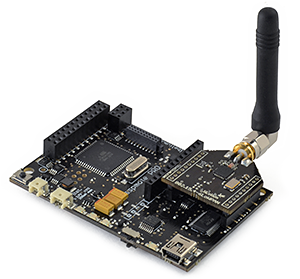
\includegraphics[scale=0.7]{images/photos/waspmote.png}
        \caption{Illustration d'une Waspmote et son antenne Zigbee.}
        \label{fig:wasp}
    \end{figure}

    
    %%%%%%%%%%%%%%%%%%%%%%%
    %%% Partie Waspmote %%%
    %%%%%%%%%%%%%%%%%%%%%%%
    \subsection{Waspmotes}
        \paragraph{}Les Waspmotes sont basées sur l'architecture ARM, plus précisément sur les modèles Arduino. En effet tout dans l'écosystème Libelium rappelle la firme bleue, de la conception des \emph{SoCs}\footnote{System on Chips, ou Système sur Puce en Français} à l'IDE. Nous retrouvons ainsi des spécifications très proches de l'\emph{Arduino Mega}~\textit{(cf. tableau \ref{tab:spec})} qui lui assure un bon compromis entre performances, possibilités d'extension et consommation.
        
        \begin{table}[h]
            \centering
            \begin{tabular}{l | l}
                \bfseries{Composant}    & \bfseries{Spécification}\tabularnewline\hline
                Microcontrôleur         & ATmega1281\tabularnewline
                Fréquence               & 14.7456~MHz\tabularnewline
                Sram                    & 8~Kio\tabularnewline
                Eeprom                  & 4~Kio\tabularnewline
                Flash                   & 128~Kio\tabularnewline
                Carte SD                & 5~Gio\tabularnewline
                Poids                   & 20~g\tabularnewline
                Température             & [-10°C ; 65°C]\tabularnewline
                Fréquence               & RTC (32~kHz)
            \end{tabular}
            \caption{Spécifications techniques de la Waspmote.}
            \label{tab:spec}
        \end{table}

        \paragraph{}Le SoC est composé de 8 Kio de SRAM (Static Random Access Memory) qui est un type de mémoire volatile qui ne nécessite pas de rafraîchissement régulier contrairement à la mémoire vive classique de nos ordinateurs. La consommation s'en trouve donc diminuée. En contre partie, les coûts de fabrication sont plus élevés. La mémoire flash de 128 Kio est utilisée pour stocker le programme de lancement du système ainsi que toutes les bibliothèques pré-compilées. Elle stocke également le programme qui était en cours d'exécution lors de l'extinction de la Waspmote. D'après la documentation, elle ne semble pas accessible au développeur. Pour palier à cela, une mémoire EEPROM (Electrically-Erasable Programmable Read-Only Memory) de 4 Kio\footnote{Les 1024 premiers octets sont réservés au système.} est disponible pour stocker des données persistantes. Ce type de mémoire permet de stocker et d'accéder aux données octet par octet contrairement à la mémoire classique qui est gérée par bloc d'octets. Elle permet d'écrire des données qui ne seront pas effacées en cas de coupure de l'alimentation. Enfin, une horloge RTC (Real Time Clock) est intégrée et permet de gérer efficacement des minuteurs et alarmes. Elle est conçue pour que la variation de son horloge interne ne dépasse pas la minute par an ($\pm$~0,16s / jour). 
        
    
        \begin{table}[h] 
            \centering
            \begin{tabular}[t]{l | l}
                \textbf{Module}			    		&	\textbf{Nb}\tabularnewline\hline
Waspmote 802.15.4 PRO           	&   6\tabularnewline
Waspmote Gateway 802.15.4       	&   2\tabularnewline
GPS Module                      	&   1\tabularnewline
GSM / GPRS Module					&	1\tabularnewline
3G + GPS Module						&	1\tabularnewline
Bluetooth							&	1\tabularnewline
Bluetooth Module PRO 5 dBi			&	1\tabularnewline
Waspmote RFID 13.56 MHz				&	1\tabularnewline
5 NFC stickers                      &	1\tabularnewline
WiFi module 5 dBi					&	1\tabularnewline

            \end{tabular}
            \hspace{1cm}
            \centering
            \begin{tabular}[t]{l | l}
                \textbf{Accessoire}					&	\textbf{Nb}\tabularnewline\hline
Rigid Solar Panel 7V – 500mA		&	2\tabularnewline
6600 mAh rechargeable battery		&	4\tabularnewline
MicroSD 2GB card pack (5 units)		&	1\tabularnewline
            \end{tabular}
            \caption{Modules de communication \& Accessoires.}
            \label{tab:modules}
        \end{table}

        \paragraph{}Cette architecture lui permet de traiter les données qui lui sont transmises par les capteurs qu'elle alimente. Sa présence est indispensable et, si chaque Waspmote peut supporter plusieurs capteurs, chaque capteur est nécessairement alimenté par une unique Waspmote.\\
        Afin de communiquer, les Waspmotes sont équipées nativement d'un module de communication auquel peut être ajouté un éventuel second module permettant de réaliser une passerelle entre deux réseaux par exemple. De part les choix effectués par Libelium, tous les modules ne sont pas disponibles au format stand-alone\footnote{À part, qui n'est pas nécessairement rattaché à un tout.} et certains sont donc exclusivement utilisable à partir de Waspmote dédiées.


    %%%%%%%%%%%%%%%%%%%%%%%
    %%% Partie Capteurs %%%
    %%%%%%%%%%%%%%%%%%%%%%%
    \subsection{Capteurs}
        \paragraph{}Les capteurs sont des composants spécialisés dépendant d'un système hôte les utilisant (les Waspmotes en l'occurrence). Chacun d'eux est sensible à un paramètre particulier (luminosité, bruit, vidéo, vent, audio\dots) dont il transmet des données brutes au système hôte. Chaque capteur est alimenté individuellement via des connecteurs qui le relie à son Waspmote.
        
        \begin{figure}[h]
            \centering
            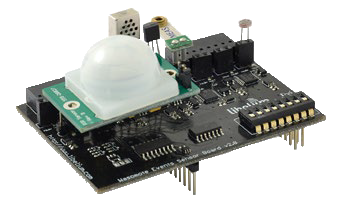
\includegraphics[scale=0.80]{images/photos/event-board-2.png}
            \caption{<< Carte capteur >> équipée entre autre de capteurs de température, de luminosité, de présence, de niveau vertical et horizontal, de présence d'eau, \textit{etc}.}
            \label{fig:capt}
        \end{figure}
        
        Si les capteurs sont conçus pour mesurer un seul paramètre, Libelium met à disposition des cartes groupant plusieurs capteurs en leur sein \textit{(voir tableau \ref{tab:capteurs} et figure \ref{fig:capt})}. Il existe plusieurs variantes de ces cartes de capteurs, chacune étant orientée pour un champs d'application spécifique. Cela permet de faciliter l'implémentation dans les cas où de nombreux capteurs auraient dû être utilisés.\\
        
        \begin{table}[h]
            \centering
            \begin{tabular}[t]{l | l}
                \textbf{Capteur}					&	\textbf{Nb}\tabularnewline\hline
Temperature sensor					&	4\tabularnewline
Humidity sensor						&	1\tabularnewline
CO sensor							&	1\tabularnewline
CO$_2$ sensor						&	1\tabularnewline
Air pollutants | sensor				&	1\tabularnewline
NO$_2$2 sensor						&	1\tabularnewline
Presence sensor (PIR)				&	1\tabularnewline
Luminosity LDR sensor				&	4\tabularnewline
Dust Sensor							&	1\tabularnewline
Ultrasound (indoor)	        		&	1\tabularnewline
Soil / Water temperature    		&	1\tabularnewline
Soil moisture sensor				&	1\tabularnewline
Solar radiation sensor				&	1\tabularnewline
Weather Station WS-3000             &	1\tabularnewline
Microphone (dBA)					&	1\tabularnewline

            \end{tabular}
            \hspace{1cm}
            \begin{tabular}[t]{l | l}
                \textbf{Carte}				    	&	\textbf{Nb}\tabularnewline\hline
Gases Board							&	2\tabularnewline
Events Board						&	2\tabularnewline
Smart Cities Board					&	1\tabularnewline
Smart Metering Board				&	1\tabularnewline
Agriculture PRO Board				&	1\tabularnewline
Prototyping Board					&	1\tabularnewline
Expansion Radio Board       		&	2\tabularnewline
            \end{tabular}
            \caption{Capteurs simples \& cartes de capteurs}
            \label{tab:capteurs}
        \end{table}
        
        \paragraph{}Dans le cadre du projet, aucune carte multi-capteurs ne semble correspondre à nos besoins, par conséquent nous utiliserons plusieurs capteurs isolés par Waspmote. De plus, ce choix permet le retrait ou l'ajout rapide de nouveaux capteurs dans le cas où les besoins viendraient à évoluer.
        
        \begin{figure}[h]
            \centering
            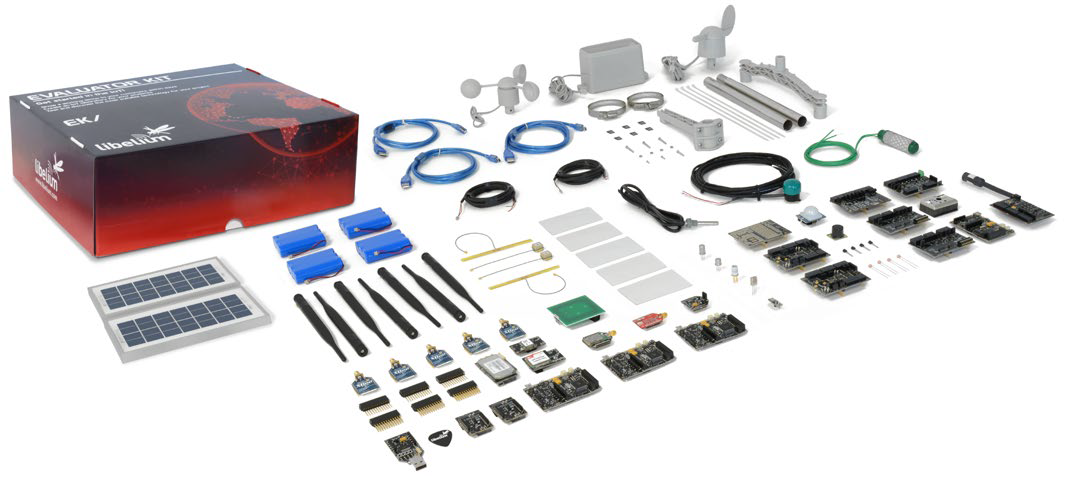
\includegraphics[scale=0.4]{images/photos/evaluator.png}
            \caption{Illustration du kit mis à disposition par le département informatique.}
            \label{fig:eval}
        \end{figure}


    
%%%%%%%%%%%%%%%%%%%%%%%%%%%
%%% Lieu d'installation %%%
%%%%%%%%%%%%%%%%%%%%%%%%%%%
\section{Lieu d'installation}
    \paragraph{}Le but final du projet est de déployer les capteurs pour former un réseau au sein de l'animalerie de la Faculté des Sciences afin de superviser les conditions des lémuriens qui y vivent. Étant donné la nature fragile des animaux, l'animalerie a été placée dans un recoin du campus universitaire, isolé au maximum des activités principales de l'université \textit{(cf. plan \ref{fig:plan})}. Par conséquent, cela ajoute plusieurs contraintes au déploiement du réseau comme par exemple l'absence de réseau Wi-Fi et Ethernet ou de prises électriques au niveau de l'animalerie.
    % Va permettre d'enchaîner avec le scénario de déploiement de façon assez fluide. Bien zob !

    \begin{figure}[h]
        \centering
        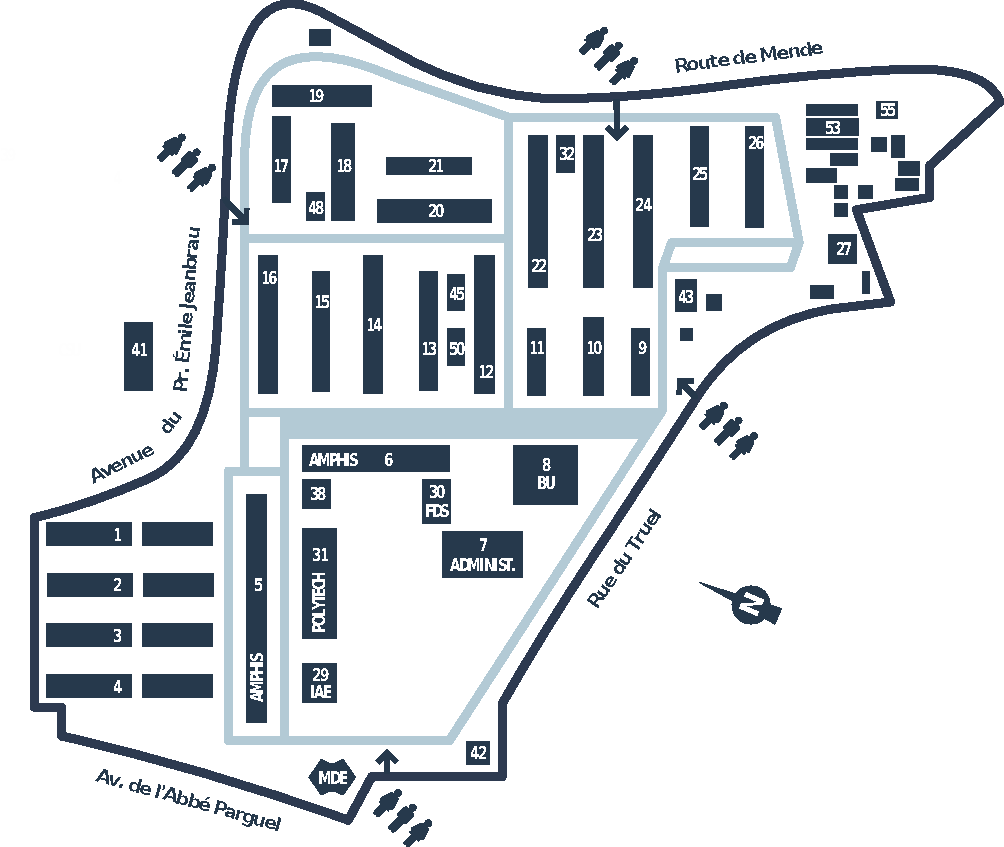
\includegraphics[trim={9.4cm 9cm 0cm 0cm},clip,scale=1.6]{images/plan.pdf}
        \caption{Plan du lieu d'installation}
        \label{fig:plan}
    \end{figure}

    \paragraph{}Sur le plan \ref{fig:plan}, l'animalerie se situe au niveau du bâtiment 53. Les données doivent être dirigées jusqu'au bâtiment 24 où se situent les chercheurs étudiant les lémuriens. Les bâtiments 25 et 26 ne possèdent pas la Wi-Fi d'après nos informations (sûr pour le bat. 25).
